\documentclass[a4paper]{article}

\usepackage[english]{babel}
\usepackage[utf8]{inputenc}
\usepackage{amsmath}
\usepackage{graphicx}
\usepackage[colorinlistoftodos]{todonotes}

\title{TTM4100 \\ Prosjektøving 1}

\author{Gruppe 31 \\\\ Bård Schjander Flugon \\ Neshat Naderi \\ Kristian Fladstad Normann \\ Stian Hegerland Hagen \\ Markus Lund \\ Kristian Bjørn Thoresen}

\date{\today}


\begin{document}
\maketitle
\clearpage

\section*{Klassediagram}
\label {sec:class}

\begin{figure}[ht]
\centering
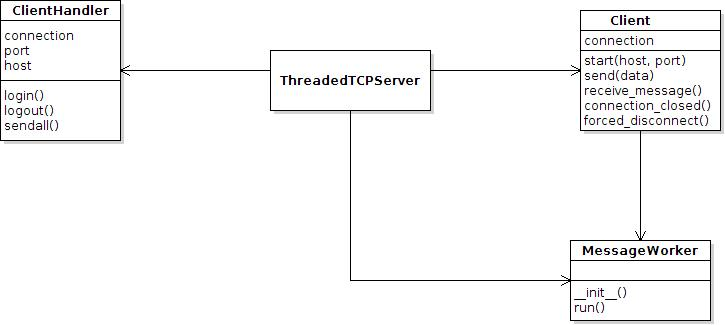
\includegraphics[width=1\textwidth]{resources/classDiag.jpg}
\caption{\label{fig:classDiag}Klassediagram}
\end{figure}

\clearpage

\section*{Sekvensdiagram}
\label{sec:sek}

\begin{figure}[ht]
\centering
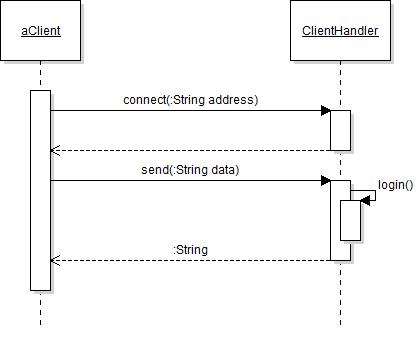
\includegraphics[width=1\textwidth]{resources/loginSeq.jpg}
\caption{\label{fig:loginSeq}Login.}
\end{figure}

\begin{figure}[ht]
\centering
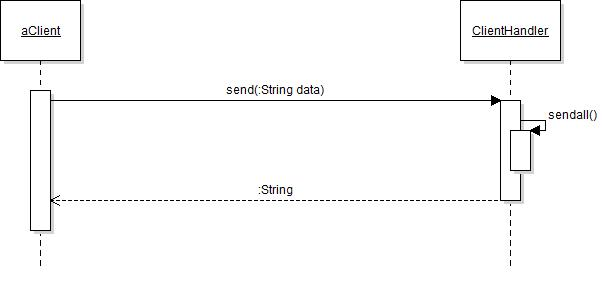
\includegraphics[width=1.3\textwidth]{resources/msgSeq.jpg}
\caption{\label{fig:msgSeq}Sende melding.}
\end{figure}

\begin{figure}[ht]
\centering
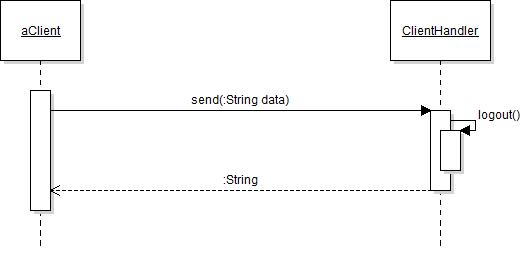
\includegraphics[width=1.2\textwidth]{resources/logoutSeq.jpg}
\caption{\label{fig:logoutSeq}Logout.}
\end{figure}
\clearpage

\section*{Tekstbeskrivelse}

Systemet vårt er bygget opp av en klient, som sender meldinger, og som samtidig kjører en messageworker som mottar meldinger fra serveren, og sier fra når det skjer. Serveren vil ta for seg å sende ut meldinger til de tilkoblede klientene, og samtidig har en clienthandler hvor har en tråd per klient, som kan motta meldinger de sender.



\end{document}
